\section{PDEBench}
{{\footnotesize
\begin{description}[labelwidth=5em, labelsep=1em, leftmargin=*, align=left, itemsep=0.3em, parsep=0em]
  \item[date:] 2022-10-13
  \item[last\_updated:] 2025-05
  \item[expired:] unkown
  \item[valid:] yes
  \item[url:] \href{https://github.com/pdebench/PDEBench}{https://github.com/pdebench/PDEBench}
  \item[domain:] CFD; Weather Modeling
  \item[focus:] Benchmark suite for ML-based surrogates solving time-dependent PDEs
  \item[keywords:]
    - PDEs
    - CFD
    - scientific ML
    - surrogate modeling
    - NeurIPS
  \item[task\_types:]
    - Supervised Learning
  \item[ai\_capability\_measured:]
    - Time-dependent PDE modeling; physical accuracy
  \item[metrics:]
    - RMSE
    - boundary RMSE
    - Fourier RMSE
  \item[models:]
    - FNO
    - U-Net
    - PINN
    - Gradient-Based inverse methods
  \item[ml\_motif:]
    - Multiple
  \item[type:] Framework
  \item[ml\_task:] Supervised Learning
  \item[notes:] Datasets hosted on DaRUS (DOI:10.18419/darus-2986); contact maintainers by email :contentReference[oaicite:6]\{index=6\}
  \item[contact.name:] Makoto Takamoto (makoto.takamoto@neclab.eu)
  \item[contact.email:] unkown
  \item[results.name:] ChatGPT LLM
  \item[results.url:] \href{unkown}{unkown}
  \item[fair.reproducible:] Yes
  \item[fair.benchmark\_ready:] Yes
  \item[ratings.software.rating:] 0
  \item[ratings.software.reason:] Not analyzed.
  \item[ratings.specification.rating:] 9.0
  \item[ratings.specification.reason:] Clearly defined PDE-solving tasks with well-specified constraints and solution formats.
  \item[ratings.dataset.rating:] 9.0
  \item[ratings.dataset.reason:] Includes synthetic and real-world PDE datasets with detailed format descriptions.
  \item[ratings.metrics.rating:] 8.0
  \item[ratings.metrics.reason:] Uses L2 error and other norms relevant to PDE solutions.
  \item[ratings.reference\_solution.rating:] 7.0
  \item[ratings.reference\_solution.reason:] Includes baseline solvers and trained models across multiple PDE tasks.
  \item[ratings.documentation.rating:] 8.0
  \item[ratings.documentation.reason:] Well-organized GitHub with examples, dataset loading scripts, and training configs.
  \item[id:] pdebench
  \item[Citations:] \cite{takamoto2024pdebenchextensivebenchmarkscientific}
  \item[Ratings:]
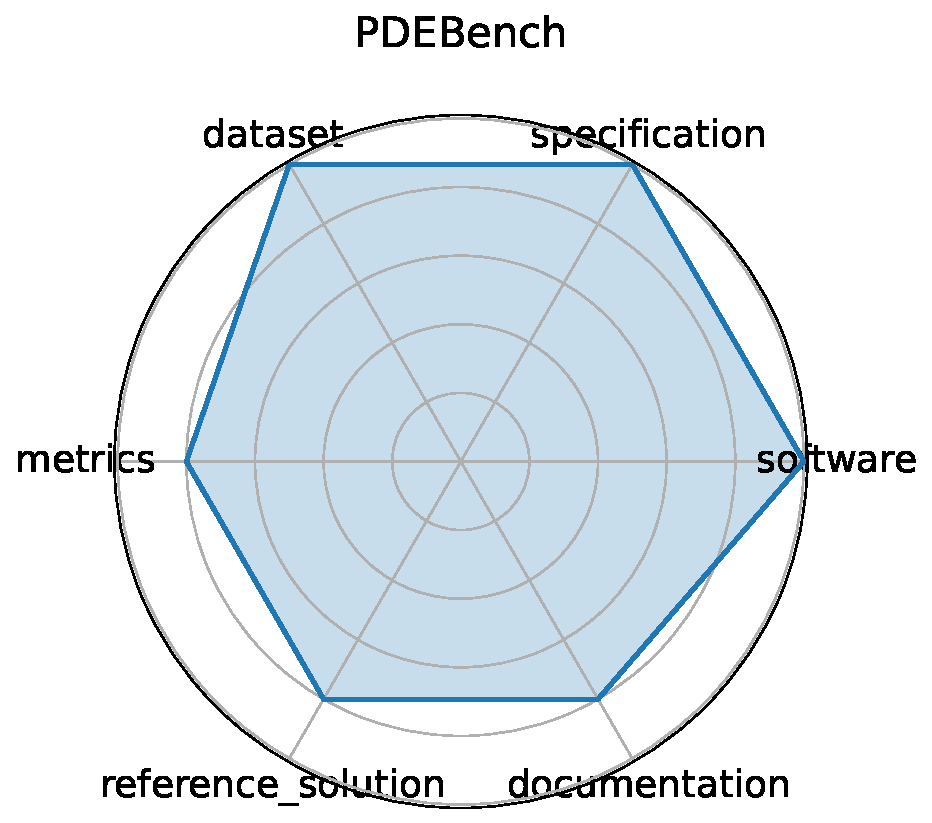
\includegraphics[width=0.2\textwidth]{pdebench_radar.pdf}
\end{description}
}}
\clearpage